\label{chapter2}

\chapter{Literature Review}

\section{Malaria}

Although the literature on malaria and related issues covers a wide variety of topics, this review will concentrate on some key topics. These topics may include malaria and its parasites, the life cycle of malaria, factors that enhance the malaria vectors, vectorial capacity and its competency,  and reviewed works(articles).\\

\noindent Malaria is  life-threatening parasitic infection spread by bites of an infected female Anopheles mosquito. \citep{odikamnoro2018incidence}. Malaria is both preventable and curable. Malaria is caused by Plasmodium parasites. Infected people usually develop symptoms 10 to 15 days after being bitten by an infected insect. Such symptoms include headache, fever, body weakness, chills, these are the most common systems that an infected person exhibits. Adults and children are also affected by malaria, but children are at a greater risk of death than adults. Malaria is a disease spread by mosquitoes. As previously noted, the vector is a female anopheles mosquito with specific traits that set it apart from other mosquito species. Anopheles mosquitos come in a variety of varieties, but only a few can transmit the parasite.  Plasmodium falciparum, Plasmodium ovale, Plasmodium malariae, Plasmodium vivax and Plasmodium knowlesi are the five malaria parasites. Plasmodium falciparum parasite, out of the five known malaria parasites, is the one that causes the majority of the global malaria load. Malaria is not always caused by all five parasites in all parts of the world. The pathogens in Ghana are Plasmodium ovale, Plasmodium malariae, and Plasmodium falciparum. Anopheles gambiae sl and Anopheles funestus are two types of Anopheles that cause malaria. In different places of the world, different kinds of Anopheles mosquitos transmit malaria.


\section{The malaria life cycle}
The Malaria parasite lifecycle begins when an infected adult female Anopheles mosquito bites to feed on human blood. It feeds on the blood of the host and releases malaria sporozoites (parasites) into the bloodstream (human being). This is the bite that causes the sickness. Parasites quickly find their way to the liver cells when they enter the human bloodstream, where they develop and multiply (schizogony). When infected liver cells break, a significant number of merozoites are released into the bloodstream, infecting red blood cells (RBCs). This stage might take anywhere between 9 and 14 days to complete. Within the RBCs, the parasites transform from "rings" to blood schizonts.After that, the schizonts burst the RBCs, releasing a swarm of merozoites that infest new RBCs. Malaria symptoms include chills and fever, which are produced by infected red blood cells rupturing. Indeed, the release of malaria parasites (merozoites) into the bloodstream from raptured RBCs corresponds to the peak of fever during malaria. The time between the infective bite and the onset of symptoms is known as the incubation period for malaria (fever, chills, etc.). Plasmodium malariae and Plasmodium vivax have a 7-14 day incubation time, however it can be shorter in Plasmodium falciparum or longer in Plasmodium malariae and Plasmodium vivax. The life cycle of malaria is depicted in the diagram below.

\begin{figure}[h]
	\centering
	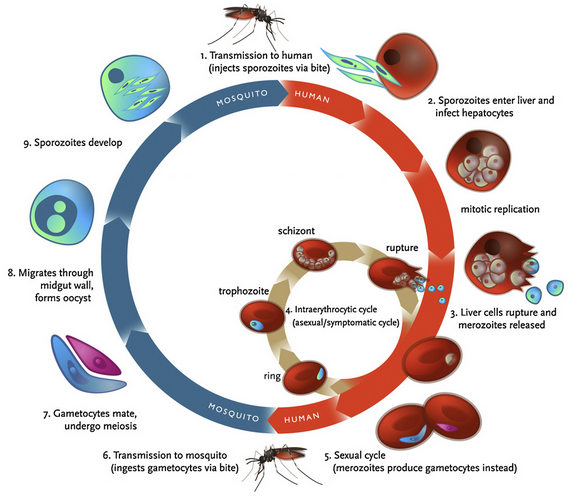
\includegraphics[scale=0.9]{life-cycle.png}
	\caption{Life cycle of malaria (Source: \url{https://cddep.org})}
	
\end{figure}


\section{Factors that enhance malaria transmission}
Malaria transmission is influenced by both climatic and non-climatic factors.
	\subsection{Climatic Factors}
Malaria is affected by three key climate conditions. They are \emph{temperature}, \emph{rainfall}, \emph{humidity}.

		\subsubsection{Temperature}
		The parasite and its vector are highly affected by temperature extremes. A parasite may take roughly 10 days to develop in the gut of a mosquito, but a lower temperature may take longer for the parasite to develop, while a higher temperature will take less time. Also, higher temperatures enhance the amount of blood meals taken and eggs laid by the vector, which result in an increase in the vector population in a given location. 	
		\subsubsection{Rainfall}
	In some circumstances, mosquitos breed in water. As a result, they frequently require the appropriate amount of rainfall to reproduce. Malaria transmission is at its peak during the rainy season, when water reservoirs that aid vector reproduction form. When it rains too much, mosquito breeding places are momentarily wiped out, but mosquitoes will begin spawning as soon as the rain stops. The life cycle of the mosquito is incompatible with several water sources. Malaria vectors thrive in stagnant water pools left over from heavy rains.
		
	
		\subsubsection{Humidity}
		Relative humidity is a measurement of the quantity of moisture in the air expressed as a percentage (0 percent humidity would mean the air is completely free of moisture and 100 percent humidity would mean the air is completely saturated with moisture). The impact of relative humidity on mosquito activity and survival on malaria transmission is significant. Mosquitoes need to live for at least 8–10 days in order to transmit malaria. High-humidity conditions are excellent for mosquitoes. They become more active when the humidity level increases. As a result, they are more active and prefer to feed at night, when the environment's relative humidity is higher.
		
		\subsection{Non-Climatic Factors}
		These are factors that influence malaria but are unrelated to the weather. The type of vectors and parasites, population movement and migration, the level of immunity in human hosts, environmental developments and urbanisation,, insecticide resistance in mosquitoes, and drug resistance in parasites are all non-climatic factors that influence the severity and incidence of malaria transmission.
		

\section{Vectorial Capacity and Competence}
The ability of the malaria vectors to transmit the disease from one person to another is defined as \textbf{"vectorial capacity"}. In contrast to the World Health Organization's definition of "vector effi-ciency," mosquito vectorial capacity is a density-dependent feature.
\textbf{"Vectorial Competence"}, which is transmissibility and susceptibility is defined as the tendency of a vector to transmit a disease or a vector's intrinsic capacity to sustain and transfer a pathogen to another host. When an infected mosquito bites a person, who is vulnerable to infection, usually refers to a vector's ability to become infected with, sustain, and transfer an infectious agent.Female mosquitoes are called vector competent when they convey the infection from one vertebrate to another during blood feeding. In arbovirus transmission, vector competence and vector capacity are both essential aspects. The intrinsic properties of the vector and pathogen, such as pathogen strain, vector strain, and pathogen genotype, are linked to this competence. The occurrence of diverse virus-vector interactions is shown by the fact that different arboviruses have variable vector competence.  

 
\textbf{}\section{Reviewed Works}
%\subsection{One}
There have been numerous studies on the malaria vector, most of which have focused on its transmission and seasonality. This work examined a number of publications or research papers in order to determine what had been done previously and what had not. For instance\\

%\subsection{Two}
\noindent \cite{ceccato2012vectorial} investigated the vectorial capacity product to track changes in potential of malaria transmission in Africa's epidemic regions. The vectorial capacity model was expanded in their research to account for the impact of rainfall and temperature variables on malaria transmission potential. They merged data from two remote sensing systems to monitor rainfall and temperature. They discovered that Eritrea has a successful malaria control program, which resulted in a significant reduction in malaria incidence between 2000 and 2009. Malaria outbreaks are still a possibility in the country due to changing weather patterns. In conclusion, the extended VCAP accurately tracks the risk of malaria in both rainy and non-rainy locations.\\


\noindent \cite{mohammadkhani2016relation} conducted study in Kerman, Iran, on the relationship between meteorological conditions and malaria incidence. Temperature was discovered to be the most effective meteorological element in the occurrence of malaria. The incidence rate grew dramatically as the mean maximum and minimum monthly temperatures increased. Finally, temperature is one of the most important climate variables influencing the occurrence of malaria, and it should be taken into account while planning for disease control and prevention.\\


%\subsection{five}
\noindent \cite{caminade2014impact} concentrated on the impact of climate change on the global spread of malaria. They used bias-corrected temperature and rainfall simulations from the Coupled Model Intercomparison Project Phase 5 climate models to compare the metrics of five statistical and dynamical malaria impact models for three future time periods (2030s, 2050s, and 2080s). The findings show that the tropical highlands' climate may become more favourable to malaria transmission in the future. Other important socioeconomic factors, such as land use change, population growth and urbanization, migratory patterns, and economic development, will need to be considered more thoroughly in future risk assessments.In conclusion, climate-induced alterations are more consistent with observed changes in a few African and South American regions. Climate change may have serious consequences in the future in the east African highlands, where a big population is at danger.\\


%\subsection{six}
\noindent \cite{christian2021effect} looked on the impact of malaria adaptive ability on subjective well-being in Ghana. They used Van Progg's (1960) theoretical framework to analyze the link between the urban and rural parts of Accra, Ghana. They discovered that in order to equalize subjective wellbeing between households with varying adopting capacity to malaria, they needed to find a way to equalize subjective welfare across households with varying adoption capacities. When compared to their counterparts with high adaptation capacity, those with low adaptive capacity demand more income. To summarize, households receiving social assistance demand a lower amount of income. Those who provide support and those who do not provide any support are compared to achieve the same degree of verbal quantification of welfare.\\

%subsection{seven}
\noindent Over an eight-year period (2001-2008), \cite{klutse2014assessment} examined climatic data and malaria cases from two ecological zones in Ghana (the transition and coastal savannah zones, respectively) to see if there was a link between malaria cases, temperature and rainfall patterns, and the potential effects of climate change on malaria epidemiological trends. The data suggest that, especially in the transition zone, maximum temperature, rather than minimum temperature or precipitation, is a better predictor of malaria trends.
 %subsection{eight}
 \cite{martens1995potential} studied on the topic of Global potential change of climate impact on Malaria Risk. They calculated the epidemic potential of a change in average temperature and rainfall patterns on malaria transmission using the UKMO-GCM model. An assessment of the possible impact of global climate change on malaria prevalence predicts a widespread increase in risk due to the extension of malaria transmission zones. Finally, the magnitude of an increase in malaria risk will be influenced by changes in malaria transmission linked to socio-economic development and the efficacy of control measures.
 %subsection{nine}
 \cite{afrane2008deforestation} studied the impact of deforestation on microclimates and Plasmodium falciparum sporogony development in Anopheles gambiae mosquitoes in a malaria-prone location of the western Kenyan highlands. P. falciparum–infected blood was given to An. gambiae mosquitos via membrane feeders. In a highland environment fed vectors were placed in dwellings in deforested areas and forested areas and parasite development was observed. When compared to wooded sites, deforested sites showed greater temperatures and relative humidity, as well as a higher overall mosquito infection rate. Sporozoites arrived 1.1 days earlier on average in deforested areas. Changes in the environment During the entire experiment period, mean indoor temperatures in experimental dwellings differed significantly between the three sites and during the entire experimental period, mean outside temperatures within the experimental dwellings differed significantly between the three sites. Changing the ecological milieu in which vectors and their parasites breed, develop, and transmit illness, whether as a result of natural events or human intervention.\\

\noindent Even though these previous research articles provide information on the transmission and capacity of malaria vectors, they mostly have limited information on the vectorial capacity or the population density of malaria vectors. Most research works are centered on how climatic factors influenced the transmission of malaria. Specifically, there is limited information on the capacity of the malaria vectors. Examining the vector population of the malaria is therefore important. Information from such study will findings give crucial research data for malaria control program implementation. Also the outcome of this study would be of much importance in contributing to achieving the Sustainable Development Goal (SDG) number 3.